\documentclass[11pt,a4paper]{article}

\usepackage[margin=1in, paperwidth=8.3in, paperheight=11.7in]{geometry}
\usepackage{amsmath,amsfonts,fancyhdr,bbm,graphicx,tikz,float,subfig}
\usetikzlibrary{automata,positioning}
\graphicspath{ {img/} }
\usepackage[section,nohyphen]{DomH}
\headertitle{Applied Deep Learning - Reviewed Notes}

\begin{document}

\title{Applied Deep Learning - Reviewed Notes}
\author{Dom Hutchinson}
\date{\today}
\maketitle

\tableofcontents\newpage

\section{Introduction}

  \begin{definition}{Deep Representation Learning}
    \textit{Representation Learning} is a set of techniques in machine learning where a system can automatically learn representations needed for feature detection from the raw data without the need for hand-designed feature descriptions. \textit{Deep Representation Learning} is then learning to classify using this feature detection.
  \end{definition}

  \begin{remark}{Biological Inspiration}
    In the natural world \textit{Neurons} are the basic working units of the brain. \textit{Neurons} can be split into three main areas
    \begin{enumerate}
      \item \textit{Dendrites} - Receives inputs from other neurons.
      \item \textit{Axon} - Carries information.
      \item \textit{Axon Terminals \& Synapses} = Send information to other neurons.
    \end{enumerate}
    \textit{Artificial Neural Networks} seek to mimic this structure.
  \end{remark}

  \begin{definition}{Neuro-Plasticity}
    \textit{Neuro-Plasticity} is the ability of a neural system to adapt its structure to accommodate new information (i.e. Learn). This can take several forms including growth \& function changes.
  \end{definition}

  \begin{proposition}{Neural Networks as an Ensemble of Sub-Networks}
    A \textit{Neural Network} can be considered to represent many \textit{sub-networks}. These sub-networks are switched between depending on which components are picked and how they are defined.
    \begin{center}
      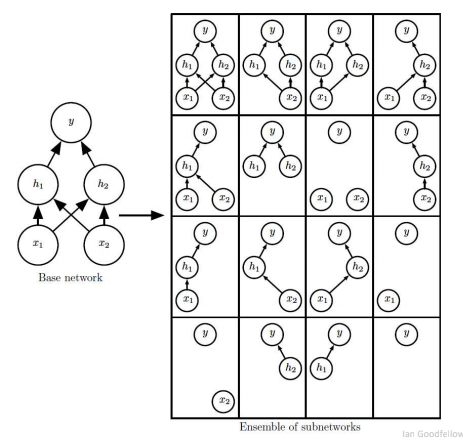
\includegraphics[width=.35\textwidth]{SubNeuralNetworks.PNG}
    \end{center}
  \end{proposition}

\section{Structures}

\subsection{Perceptron}

  \begin{definition}{Perceptron}
    A \textit{Perceptron} is an algorithm for supervised learning of a binary classifier. A \textit{Perceptron} defines a hyperplane which acts as a decision boundary which linearly separates the input-state space. These two regions correspond to the two-classes. A perceptron has the following structure.

    \begin{center}\begin{tikzpicture}
      % nodes
      \node         at (-2,0)      {$\text{bias}\big\{$};
      \node[circle] at (0,0)  (x0) {$x_0:=-1$};
      \node[circle] at (0,-1) (x1) {$x_1$};
      \node[circle] at (0,-2) (x2) {$x_2$};
      \node         at (0,-3) (x3) {$\vdots$};
      \node[circle] at (0,-4) (xk) {$x_k$};
      \node         at (0,1)       {$\overbrace{}^{\text{input}}$};

      \node[rectangle] at (3,-2) (sum) {\huge $\Sigma$};
      \node            at (3,1)       {$\overbrace{}^{\text{weighted sum}}$};
      \node[rectangle] at (6,-2) (act) {\huge $g$};
      \node            at (6,1)       {$\overbrace{}^{\text{activation function}}$};
      \node[rectangle] at (9,-2) (out) {\huge $y\in\{-1,1\}$};
      \node            at (9,1)       {$\overbrace{}^{\text{output}}$};

      % edges
      \path[->]
      (x0) edge node[above] {$w_0$} (sum)
      (x1) edge node[above] {$w_1$} (sum)
      (x2) edge node[above] {$w_2$} (sum)
      % (x3) edge (sum)
      (xk) edge node[above] {$w_k$} (sum)
      (sum) edge (act)
      (act) edge (out);
    \end{tikzpicture}\end{center}
    \begin{itemize}
      \item[$x_0$] is the bias element. It is always set to $-1$ in the input and the actual value is defined by its weight $w_0$.
      \item[$\pmb{x}=(x_0,\dots,x_k)$] is the input. Note that $x_0$ is the bias and  $(x_1,\dots,x_k)$ are the observed inputs.
      \item[$\pmb{w}=(w_0,\dots,w_k)$] is the weights assigned to each input (including the bias).
      \item[$\Sigma$] is the weighted sum of the bias \& inputs. $\displaystyle\Sigma:=\sum_{i=0}^kw_ix_i=\pmb{w}^T\pmb{x}$
      \item[$g$] is the \textit{Activation Function} which maps the result from the weighted sum $\Sigma$ to $\{-1,1\}$, performing a binary classification.
      \item[$y$] is the output of the \textit{Activation function}. (i.e. the classification). Typically denoted as $f(\pmb{x};\pmb{w})$ \[ y=g\left(\sum_{i=0}^kx_iw_i)\right)=g(\pmb{w}^T\pmb{x})\]
    \end{itemize}
  \end{definition}

  \begin{remark}{Limitations of Perceptron}
    A \textit{Perceptron} can only perform linear binary classification so is not useful when two classes are not linearly separable.
  \end{remark}

  \begin{proposition}{Perceptron Supervised Learning Rule}
    To make a perceptron learn from misclassifications, we adjust the weight vector $\mathbf{w}$. One learning rule for this is to update the current weights by a certain proportion of the error made $\Delta \mathbf{w}$.
    \[ \pmb{w}_{t+1}=\pmb{w}_t+\Delta\pmb{w}\quad\text{where}\quad\Delta\pmb{w}=\begin{cases}\eta f^*(\pmb{x})\pmb{x}&\text{if }\overbrace{f^*(\pmb{x})}^\text{ground truth}\neq \overbrace{f(\pmb{x})}^\text{prediction}\\0&\text{otherwise}\end{cases}\]
    where $\eta\in\reals^+$ is the \textit{Learning Rate}. Remember that $f^*(\cdot)\in\{1,-1\}$.
  \end{proposition}

  \begin{remark}{Learning Rate $\eta$}
    The \textit{Learning Rate} $\nu$ defines how big the steps learning rule makes towards a minimum. The \textit{Learning Rate} needs to be tuned as too small a value will mean it takes a long time (and a lot of data) to reach a minimum, whereas too great a value means the minimum can be overstepped and convergence is unlikely.
  \end{remark}

  \begin{proposition}{Training Process for a Single-Layer Perceptron}
    Let $\left\{\big(\pmb{x}_1,f^*(\pmb{x}_1)\big),\dots,\big(\pmb{x}_N,f^*(\pmb{x}_N)\big)\right\}$ be a set of training data.
    \par The following is an algorithm for learning a good set of weights $\pmb{w}$ for a \textit{Perceptron}
    \begin{enumerate}
      \item Initialise the weight vector $\pmb{w}=\pmb0$
      \item Consider next training datum $\big(\pmb{x}_i,f^*(\pmb{x}_i)\big)$.
      \item Calculate prediction $f(\pmb{x}):=g(\mathbf{w}^T\mathbf{x})$.
      \item Compare prediction $f(\pmb{x})$ and ground truth $f^*(\pmb{x})$.
      \item Update the weight vector $\pmb{w}=\pmb{w}+\Delta\pmb{w}\quad\text{where}\quad\Delta\pmb{w}=\begin{cases}\eta f^*(\pmb{x})\pmb{x}&\text{if }f^*(\pmb{x})\neq f(\pmb{x})\\0&\text{otherwise}\end{cases}$
      \item Repeat ii)-v) until the training set is exhausted.
    \end{enumerate}
  \end{proposition}

  \begin{remark}{Arbitrary Decision Boundaries}
    Multiple preceptrons can be connected to form networks which are able to define arbitrary decision boundaries, rather than just a linear boundary. See \texttt{Section 4} for details on these network architectures.
  \end{remark}

\subsubsection{Activation Functions}

  \begin{proposition}{Activation Function}
    There are several choice for the \textit{Activation Function} including:
    \begin{itemize}
      \item The \textit{Sign} activation function binarily assigns values depend on whether they are positive or negative. \textit{Sign} is not differentiable.
      \[ g_{sign}(x):=\begin{cases}1&x\geq0\\-1&x<0\end{cases}=\frac{x}{|x|} \]

      \item The \textit{Rectifying Linear Unit} (ReLU) function is a differentiable activation function.
      \[\begin{array}{rcl}
          g_{ReLU}(s)&:=&\max\{0,s\}\\
          g_{ReLU}'(s)&:=&\begin{cases}1&\text{if }s\geq0\\0&\text{otherwise}\end{cases}
      \end{array}\]
    \end{itemize}
  \end{proposition}

  \begin{remark}{Limitation of ReLU}
    Using \textit{ReLU} introduces a problem of \textit{Dying Neurons} where a large gradient flowing through \textit{ReLU} may force the neuron never to activate again (as it pushes the incoming signal to 0). This is bad, as these neurons will no longer contribute to learning anymore.
  \end{remark}

\subsection{Artificial Neural Network}

  \begin{figure}[ht!]
    \centering
    \tikzstyle{block} = [rectangle, draw, fill=blue!20, text width=5em, text centered, rounded corners, minimum height=4em]
    \begin{tikzpicture}[node distance = 3cm, auto]
      \node [block] (input) {Input Layer};
      \node [block, right of=input] (hidden1) {Hidden Layer 1};
      \node [block, right of=hidden1] (hidden2) {$\dots$};
      \node [block, right of=hidden2] (hidden3) {Hidden Layer K};
      \node [block, right of=hidden3] (output) {Output Layer};

      \draw[->] (input) edge (hidden1);
      \draw[->] (hidden1) edge (hidden2);
      \draw[->] (hidden2) edge (hidden3);
      \draw[->] (hidden3) edge (output);
    \end{tikzpicture}
    \caption{Abstract Diagram of the Structure of an Artifical Neural Network with $K$ hidden layers.}
    \label{fig:ANN}
  \end{figure}

  \begin{definition}{Artificial Neural Network}
    An \textit{Artificial Neural Network} is a graph which loosely models the neural network of a brain and is used for classification/regression.
    \par An \textit{Artificial Neural Network} is structured as a set of layers with each layer only takes input from the layer immediately before, and passes its signal to the layer immediately after. There are three groups of layers:
    \begin{enumerate}
      \item Input Layer. Observed values.
      \item Hidden Layer\underline{s}. A collection of perceptrons which are grouped into layers. How the layers pass their output/take an input is defined by the architecture of the neural network
      \item Output Layer. The classification of the network. This may be a single node which represents a numerical value being predicted, or a collection of $N$ nodes used to classify to one of $N$ classes.
    \end{enumerate}
    See \texttt{Figure \ref{fig:ANN}} for an diagram of the structure of an ANN.
  \end{definition}

  \begin{definition}{Forward Propagation}
    \textit{Forward Propagation} is the process a neural network calculating its output, once it is given a set of inputs.
    \par This is done by inserting the observed values into the correct nodes of the input layer. This values are then passed forwards, throught the network, one hidden layer at a time. The flow of data is unidirectional.
    \par Several values are calculated during \textit{Forward Propagation}
    \begin{itemize}
      \item Signal $s_j^l:=(w^l)^Tf^{l-1}$. The weighted sum calculated by the perceptron from its inputs, before it is passed to the activation function.
      \item Output $f_j^l:=g_j^l(s_j^l)$. The result from applying the activation function $g^j_l$ to the signal $s_j^l$.
    \end{itemize}
    Here $l$ denotes a layer and $j$ the specific node in that layer.
  \end{definition}

\section{Deep Neural Networks}

  \begin{definition}{Deep Neural Network}
    A \textit{Deep Neural Network} is an \textit{Artifical Neural Network} with multiple hidden layers. These multiple hidden layers allow \textit{Deep Neural Networks} to learn complex non-linear relationships as later layers can compose features identified by earlier layers.
  \end{definition}

\subsection{General}

\subsubsection{Usefulness}

  \begin{remark}{Advantages of Deep Neural Networks}
    Here are some advantages \textit{DNNs} offer over neural networks with a single hidden layer.
    \begin{itemize}
      \item \textit{Hierarchical Automatic Modularisation}. A deep neural network has many layers, and the information of each layer is available to the succeeding layer. This means each layer can be considered to extract slightly more precise features (e.g. pixel colours $\to$ edges $\to$ corners $\to$ object parts $\to$ object class). These modular layers are generated automatically during training.
      \item \textit{Practical Performance}. Greater depth gives greater performance than greater width. Note that large networks (either by width or depth) require more training time and larger data sets.
      \item \textit{The Oscillation Argument}. There are functions $f$ that can be represented by a \underline{deep} ReLU network with a polynomial number of neurons, whereas a \underline{shallow} network would require exponentially many units.
    \end{itemize}
  \end{remark}

\subsubsection{Overfitting}

  \begin{figure}[H]
    \centering
    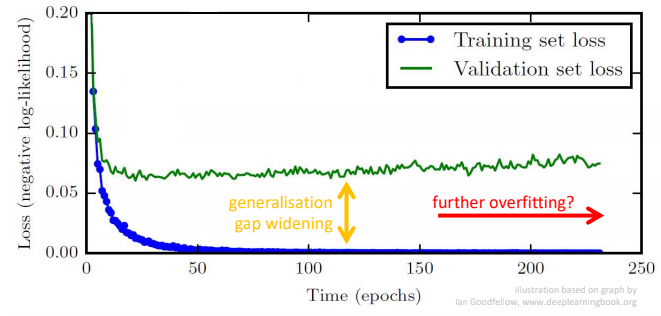
\includegraphics[width=.7\textwidth]{overfitting.PNG}
    \caption{An example of a bad relationship between training and testing loss}
    \label{fig:Overfitting}
  \end{figure}

  \begin{proposition}{Overfitting}
    \textit{Deep Neural Networks} have lots-and-lots of parameters, meaning they have high degrees of freedom and thus prone to \textit{Overfitting} (ie the model is fitted too closely to the training data and does not fit unseen data well).
    \par \texttt{Figure \ref{fig:Overfitting}} provides an example of how \textit{Overfitting} can be identified graphically as the distance between training and testing loss increases with each time step, and the training loss converges to zero. Ideally the lines for training and testing loss would be fairly similar.
    \par \textit{Overfitting} can be combatted by: Using more data; Using data which represents the full sample space better; And, strategic sampling of data.
  \end{proposition}

  \begin{definition}{Data Augmentation}
    Collecting data can be expensive and hard. \textit{Data Augmentation} is a set of techniques to increase the available set of data, without having to collect more data, by slightly modifying already observed data. For images this may involve: cropping; translating; adding noise; shifting the hue...
  \end{definition}

  \begin{definition}{Regularisation}
    A \textit{Regularisation} is any modification made to a learning algorithm which is intended to reduced its \textit{generalisation error}, \underline{but} not its \textit{training error}. This is typically done by introducing more information and making changes to the \textit{Loss Function}.
    \begin{itemize}
      \item[\textit{$L$-Regularisation}] places constraints on the weight space, thus reducing the searchable area for the model.
      \item[\textit{$L_1$-Regularisation}] extends the cost function $J(\cdot,\cdot)$ to include a sum of the absolute values of all the weights, with a dampening factor $\lambda$.
      \par This gives the following cost function $J_{L1}$ and weight update rule
      \everymath={\displaystyle}
      \[\begin{array}{rrl}
        J_{L1}(X;W)&:=&J(X,W)+\lambda\sum_{w\in W}|w|\\
        W^l&\leftarrow&W^l-\eta\left(\nabla J+\lambda\cdot\mathtt{sign}(W^l)\right)
      \end{array}\]
      \item[\textit{$L_2$-Regularisation}] extends the cost function $J(\cdot,\cdot)$ to include a sum of the square value of each weights, with a dampening factor $\lambda$.
      \par This gives the following cost function $J_{L2}$ and weight update rule
      \everymath={\displaystyle}
      \[\begin{array}{rrl}
        J_{L2}(X;W)&:=&J(X,W)+\frac\lambda2\sum_{w\in W}w^2\\
        W^l&\leftarrow&W^l-\eta\left(\nabla J+\lambda W^l\right)
      \end{array}\]
    \end{itemize}
  \end{definition}

  \begin{remark}{$L_1$ Regularisation vs $L_2$ Regularisation}
    Both \textit{$L_1$ Regularisation} and \textit{$L_2$ Regularisation} encourage the model to learning the smallest-valued set of weights which minimise the normal cost function. Moreover, they discourage extreme weight values.
    \par The key difference is that, in \textit{$L_1$ Regularisation} the less important features are shrunk to zero, removing that feature altogether.
  \end{remark}

  \begin{definition}{Dropout}
    \textit{Dropout} is a training procedure which builds on the idea that \textit{Neural Networks} are an ensemble of sub-networks (See \texttt{Proposition 1.1}) and seeks to allow each sub-network to train somewhat independently.
    \par \textit{Dropout} does this by, each training loop, choosing a random set of nodes and setting the inbound weight to each of these nodes to 0. This effectively immobilises this set of nodes during this training loop
    \par During validation all weights are turned on, so the output of the network is significantly greater. To combat this weights are set to $pW$ in order to reduce their magnitude (where $p$ is the probability of a particular node being immobilised in a particular training loop).
  \end{definition}

  \begin{definition}{DropConnect}
    \textit{DropConnect} is a variation on \textit{Dropout} where \underline{connections} are dropped, rather than nodes. This a more fine-grained approach to ensemble learning than \textit{Dropout}.
  \end{definition}

\subsubsection{Extensions}

  \begin{proposition}{Extensions of Neural Networks}
    Here I suggest some areas which could be explored to extend implementation of \textit{Neural Networks}
    \begin{itemize}
      \item Learn an ensemble of deep networks and then compress them into a single shallow-network. (This is sometimes possible).
      \item Learn a set of networks which each deal with a specific subtask of the problem and then learn another network whcih decides which of these specialised networks (or which combination) to use.
    \end{itemize}
  \end{proposition}

\subsection{Fully Connected DNN}

  \begin{definition}{Fully Connected DNN}
    A \textit{Fully Connected DNN} is an \textit{Artificial Neural Network} where each node in a layer takes an input from \underline{every} node in the preceding layer and passes its output to \underline{every} node in the next layer.
    \par The output of each perceptron is the weighted sum of its inputs, passed through an activation function.
    \par Below is a diagram of a MLP of \textit{depth} $N$ (i.e. there are $N$ layers of computation)
    \begin{center}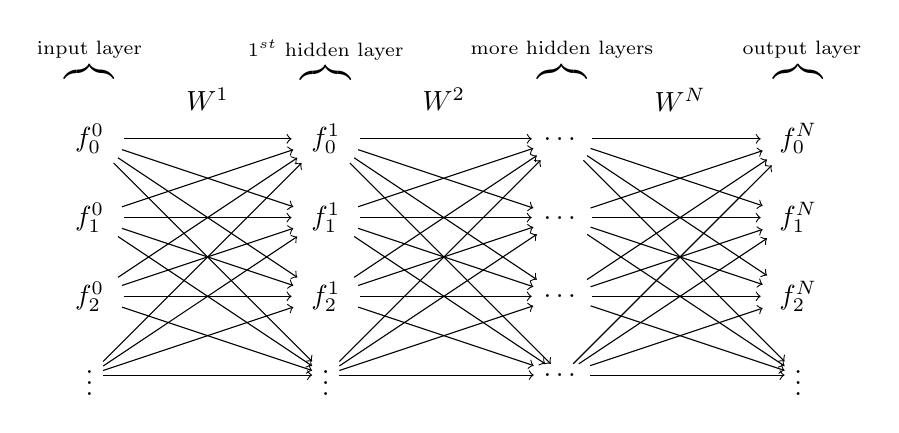
\begin{tikzpicture}
      % nodes
      \node         at (0,1)        {$\overbrace{}^{\text{input layer}}$};
      \node[circle] at (0,0)  (f00) {$f^0_0$};
      \node[circle] at (0,-1) (f01) {$f^0_1$};
      \node[circle] at (0,-2) (f02) {$f^0_2$};
      \node         at (0,-3) (f0)  {$\vdots$};
      \node         at (1.5,.5)(w1)  {$W^1$};

      \node         at (3,1)        {$\overbrace{}^{1^{st}\text{ hidden layer}}$};
      \node[circle] at (3,0)  (f10) {$f^1_0$};
      \node[circle] at (3,-1) (f11) {$f^1_1$};
      \node[circle] at (3,-2) (f12) {$f^1_2$};
      \node         at (3,-3) (f1)  {$\vdots$};
      \node         at (4.5,.5)(w2)  {$W^2$};

      \node         at (6,1)        {$\overbrace{}^\text{more hidden layers}$};
      \node[circle] at (6,0)  (f20) {$\dots$};
      \node[circle] at (6,-1) (f21) {$\dots$};
      \node[circle] at (6,-2) (f22) {$\dots$};
      \node         at (6,-3) (f2)  {$\dots$};
      \node         at (7.5,.5)(wN)  {$W^N$};

      \node         at (9,1)        {$\overbrace{}^{\text{ output layer}}$};
      \node[circle] at (9,0)  (fN0) {$f^N_0$};
      \node[circle] at (9,-1) (fN1) {$f^N_1$};
      \node[circle] at (9,-2) (fN2) {$f^N_2$};
      \node         at (9,-3) (fN)  {$\vdots$};

      % edges
      \path[->]
      % input layer
      (f00) edge (f10)
      (f00) edge (f11)
      (f00) edge (f12)
      (f00) edge (f1)

      (f01) edge (f10)
      (f01) edge (f11)
      (f01) edge (f12)
      (f01) edge (f1)

      (f02) edge (f10)
      (f02) edge (f11)
      (f02) edge (f12)
      (f02) edge (f1)

      (f0) edge (f10)
      (f0) edge (f11)
      (f0) edge (f12)
      (f0) edge (f1)
      % first hidden layer
      (f10) edge (f20)
      (f10) edge (f21)
      (f10) edge (f22)
      (f10) edge (f2)

      (f11) edge (f20)
      (f11) edge (f21)
      (f11) edge (f22)
      (f11) edge (f2)

      (f12) edge (f20)
      (f12) edge (f21)
      (f12) edge (f22)
      (f12) edge (f2)

      (f1) edge (f20)
      (f1) edge (f21)
      (f1) edge (f22)
      (f1) edge (f2)

      % output layer
      (f20) edge (fN0)
      (f20) edge (fN1)
      (f20) edge (fN2)
      (f20) edge (fN)

      (f21) edge (fN0)
      (f21) edge (fN1)
      (f21) edge (fN2)
      (f21) edge (fN)

      (f22) edge (fN0)
      (f22) edge (fN1)
      (f22) edge (fN2)
      (f22) edge (fN)

      (f2) edge (fN0)
      (f2) edge (fN1)
      (f2) edge (fN2)
      (f2) edge (fN);
    \end{tikzpicture}\end{center}
    Note that each layer can have a different number of nodes (AKA \textit{width}).
    \par For each consecutive pair of layers $\pmb{f}^i,\pmb{f}^j$ (of widths $n_i,n_j$ respectively) there is an associated weight matrix $W\in\reals^{n_i\times n_j}$ st $\pmb{f}^j=W^T\pmb{f}^i$.
  \end{definition}

  \begin{remark}{Discriminating Power of Differt Depth Fully Connected DNNs}
    A \textit{Fully Connected DNN} with a \underline{single} hidden layer is sufficient to represent any boolean or continuous function, althought the layer may be exponentially wider than the input.
    \par A \textit{Fully Connected DNN} with \textit{two} hidden layers is sufficient to represent any mathematical function.
  \end{remark}

  \begin{proposition}{MLPs as Computation Graphs}
    \[\begin{array}{rrrll}
      &s_i^j&:=&(W^j)^Tf^{j-1}&\tiny\text{weighted sum of the $i^{th}$ node of the $j^{th}$ hidden layer}\\
      \implies&\dfrac{\partial s_i^j}{\partial w_{ii}^j}&=&f_i^{j-1}\\
      &f_i^j&:=&g_i^j(s_i^j)&\tiny\text{$i^{th}$ output vajue of $j^{th}$ hidden layer}\\
      \implies&\dfrac{\partial f_i^j}{\partial s_i^j}&=&\text{depends on def of }g_i^j
    \end{array}\]
  \end{proposition}

  \begin{proposition}{Output Layer for Classification Problem}
    When using a \textit{Fully Connected DNN} for classification the output layer represents a probability distribution for each possible class. This means, in the output layer, the node values are in $[0,1]$ and they sum to $1$.
    \par This distribution is achieved by using a \textit{Softmax Neuron Group} in the last layer with activation function. Defined as
    \[  g_j^N(s_j^N):=\frac{e^{s_j^N}}{\displaystyle\sum_{i\in\text{Group}}e^{s_i^N}} \]
    This has gradients
    \[\begin{array}{rcl}
      g'_j^N(s_j^N)&=&f_j^N(1-f_j^n)\\
      g'_j^N(s_{i}^N)&=&-f_j^Nf_i^N\quad\text{for }i\neq j
    \end{array}\]
  \end{proposition}

\subsection{Convolution Connected DNN}

  \begin{remark}{This is actually the Cross-Correlation operation, but is what is used in practice.}
    Convolution flips the kernel.
  \end{remark}

  \begin{definition}{Channels}
    When we have multiple data readings per instance (e.g. for each pixel of an RGB image) we consider each of these data fields to be a \textit{channel}. When we apply a convolution they must have the same dimension as the number of channels, and they can applied to both space \& channels.
  \end{definition}

  \begin{definition}{Convolution DNN (CNNs)}
    A \textit{Convolution DNN} is an \textit{Artificial Neural Network} contains a \textit{Convolutional Layer} (it may also contain fully connected layers). \textit{Pooling Layers} are common in CNNs in order to reduce dimensionality.

    \begin{itemize}
      \item A \textit{Convolutional Layer} takes an $n$-dimensional grid-like topology (e.g. an image or video) as an input and applies several convolutions to this input (rather than matrix multiplication). The output from the convolution in each position of the input is passed through an \textit{Activation Funtion} and then to the node in the layer at the equivalent position. The convolutional layer is three dimensional with $X,Y$ representing spatial data and $Z$ the convolution applied.
      \par A \textit{Convolutional Layer} has two possible additions \textit{Zero Padding} and \textit{Stride Length}. See \texttt{Definition 4.4} and \texttt{Definition 4.5}.
      \item A \textit{Pooling Layer} takes an $n$-dimensional grid-like topology as an input and for each position it outputs a summary of the values in the neighbourhood of that position. This summary is typically the: mean, min or max value; and the size of the neighbourhood is user defined.
      \par \textit{Pooling} is applied after the convolution and the activation function, and reduces the output size.
    \end{itemize}
    Rather than fitting/learning a weights matrix, here we are learning the \textit{Kernel} (AKA \textit{Tensor}) of the convolution.
  \end{definition}

  \begin{definition}{Zero Padding}
    The output from \textit{Convolution} is smaller than the original input. This is bad as eventually the dataset would disappear. To avoid this \textit{Zero Padding} is used. \textit{Zero Padding} adds rings zeros to the outside of the input st the input and output are the same size after \textit{Convolution} is applied.
    \par The number of rings added depends on the size of the Kernel. For a Kernel of size $N\times M$: $M-1$ rows are added to the top \& bottom of the input; and, $N-1$ columns are added to the left and right of the input.
  \end{definition}

  \begin{definition}{Stride Length}
    \textit{Stride Length} defines how far the convolution operation steps each time. This applies to both horizontal and vertical steps. The greater the \textit{Stride Length}, the smaller the output will be.
    \par In practice \textit{Stride Length} is rarely set to one as this requires a lot more weights to be fitted and often little is gained by looking at values which are adjacent.
  \end{definition}

  \begin{figure}[ht!]
    \centering
    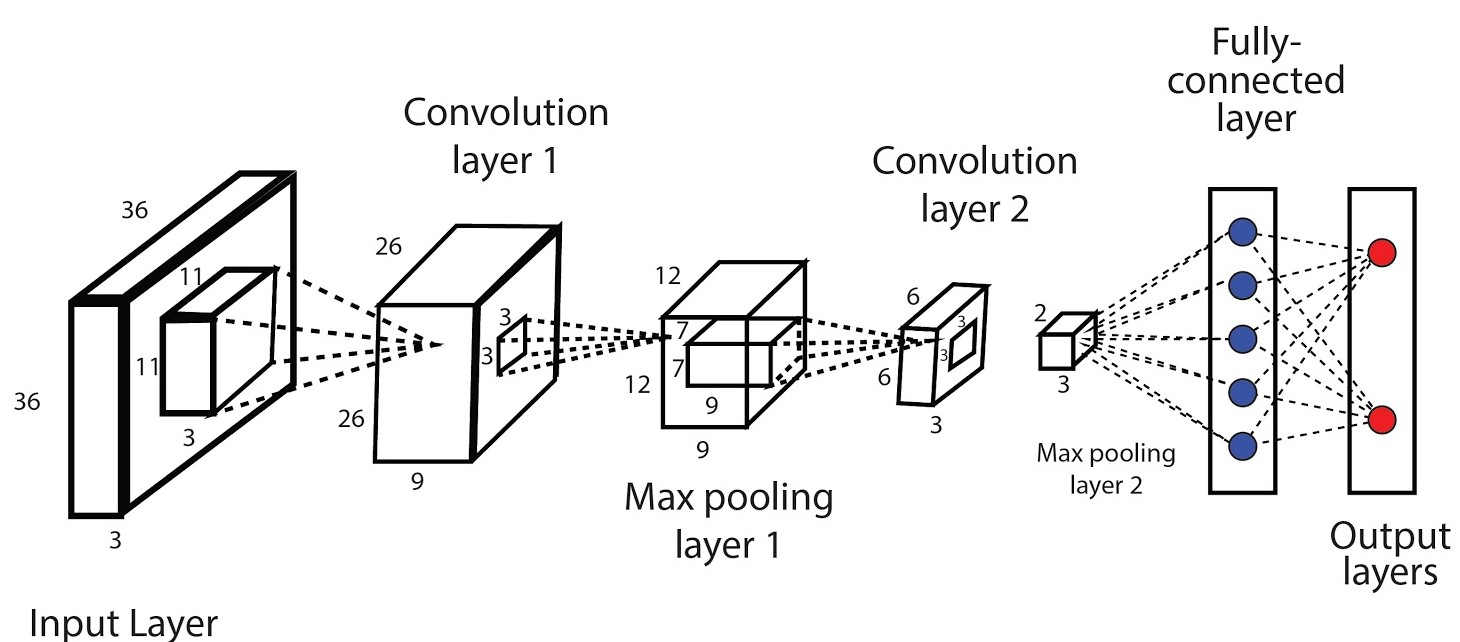
\includegraphics[width=.5\textwidth]{CNNArchitectureDiagram.jpg}
    \caption{Example of an Architecture for a Convolution DNN}
    \label{fig:CNN}
  \end{figure}

  \begin{example}{CNN Architecture}
    \texttt{Figure \ref{fig:CNN}} gives an example of an architecture for a convolution DNN. In this example
    \begin{itemize}
      \item \textit{Input Layer} has dimension $36\times36\times3$. This could be an RGB image with $36\times36$ pixels.
      \item \textit{Convolution Layer 1} applies 9 different convolutions, each with a kernel of dimension $11\times11\times3$. In this example a stride of 1 is used and no zero-filtering. This means the output has dimension $26\times26$ and a depth of $9$ (due to 9 convolutions being used).
      \item \textit{Max Pooling Layer 1} applies the max pooling operation to each  $3\times3\times1$ set of values in \textit{Convolution Layer 1}. In this example a stride of 2 is used, meaning the output has dimension $12\times12\times9$.
      \item \textit{Convolution Layer 2} applies 3 different convolutions, each with a kernel of dimension $7\times7\times9$.
      \item \textit{Max Pooling Layer 2} applies the max pooling operation to each $3\times3\times1$ set of values in \textit{Convolution Layer 2}.
      \item A \textit{Fully-Connected Layer} is the used before the final classification.
    \end{itemize}
  \end{example}

  \begin{remark}{Attraction of CNNs}
    Here are some features which distinguish \textit{Convolution Layer}s away from \textit{Fully Connect Layer}s
    \begin{enumerate}
      \item \textit{Sparse Interactions}. In CNNs a node in one layer does not necessarily connected to every node in the next layer. This means that changing this node will not affect every node in the next layer. This is ideal due to the grid structure of the input, where there is implicit relationships between adjacent cells/cell groups (e.g. adjacent pixels in an image).
      \item \textit{Parameter Sharing}. The same parameter/weight is used for more than one function in the network. This can be considered as tying two parameters together st that have the same value. We use prior knowledge to decide which nodes to tie together (rather than doing it randomly). This reduces the number of parameters which need to be optimised (which means less data is required for training). The number of reduced parameters increases for later layers. This does not affect the runtime of the forward pass, but significantly reduces the memory requirements of the model. %TODO
      \item \textit{Equi-variant Representations}. If the input changes/shifts in a certain way (e.g. translation), then the output changes in exactly the same way. This is as a result of the previous two properties. However, CNNs are \underline{not} equivariant to rotation or scaling.
    \end{enumerate}
  \end{remark}

  \begin{remark}{Implementing CNNs}
    In practice there are several difficulties in implementing CNNs, including
    \begin{itemize}
      \item Care needs to be taken when backpropagating CNNs with zero padding or stride greater than 1.
    \end{itemize}
  \end{remark}

  \begin{remark}{Training CNNs}
    \begin{itemize}
      \item The most expensive part of training CNNs is training the convolutional layers. The fully-connected layers at the end are relatively inexpensive as they have a small number of features.
      \item When performing gradient descent, every gradient step requires a complete run of feed-forward propagation and backward propagation through the entire network.
    \end{itemize}
  \end{remark}

\subsubsection{Residual Networks (ResNets)}

  \begin{figure}[ht!]
    \centering
    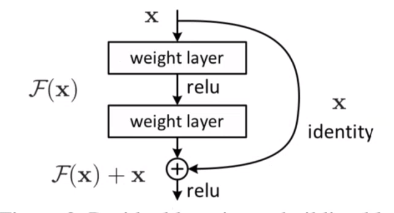
\includegraphics[width=.35\textwidth]{ResNet.PNG}
    \caption{Example of a Residual Network Layer}
    \label{fig:ResNet}
  \end{figure}

  \begin{proposition}{Residual Networks (ResNet)}
    \textit{ResNets} are a version in CNNs where filters are applied to the input and then merged back (using addition) with the input before being passed to the activation function. This leads to faster convergence by searching for weights which deviate only slightly from the identity. This allows for deeper networks.
    \par See \texttt{Figure \ref{fig:ResNet}} for an example of the architecture of a \textit{ResNet} layer.
  \end{proposition}

\subsection{Recurrent DNN}

TODO

\section{Algorithms}

  \begin{figure}[H]
    \centering
    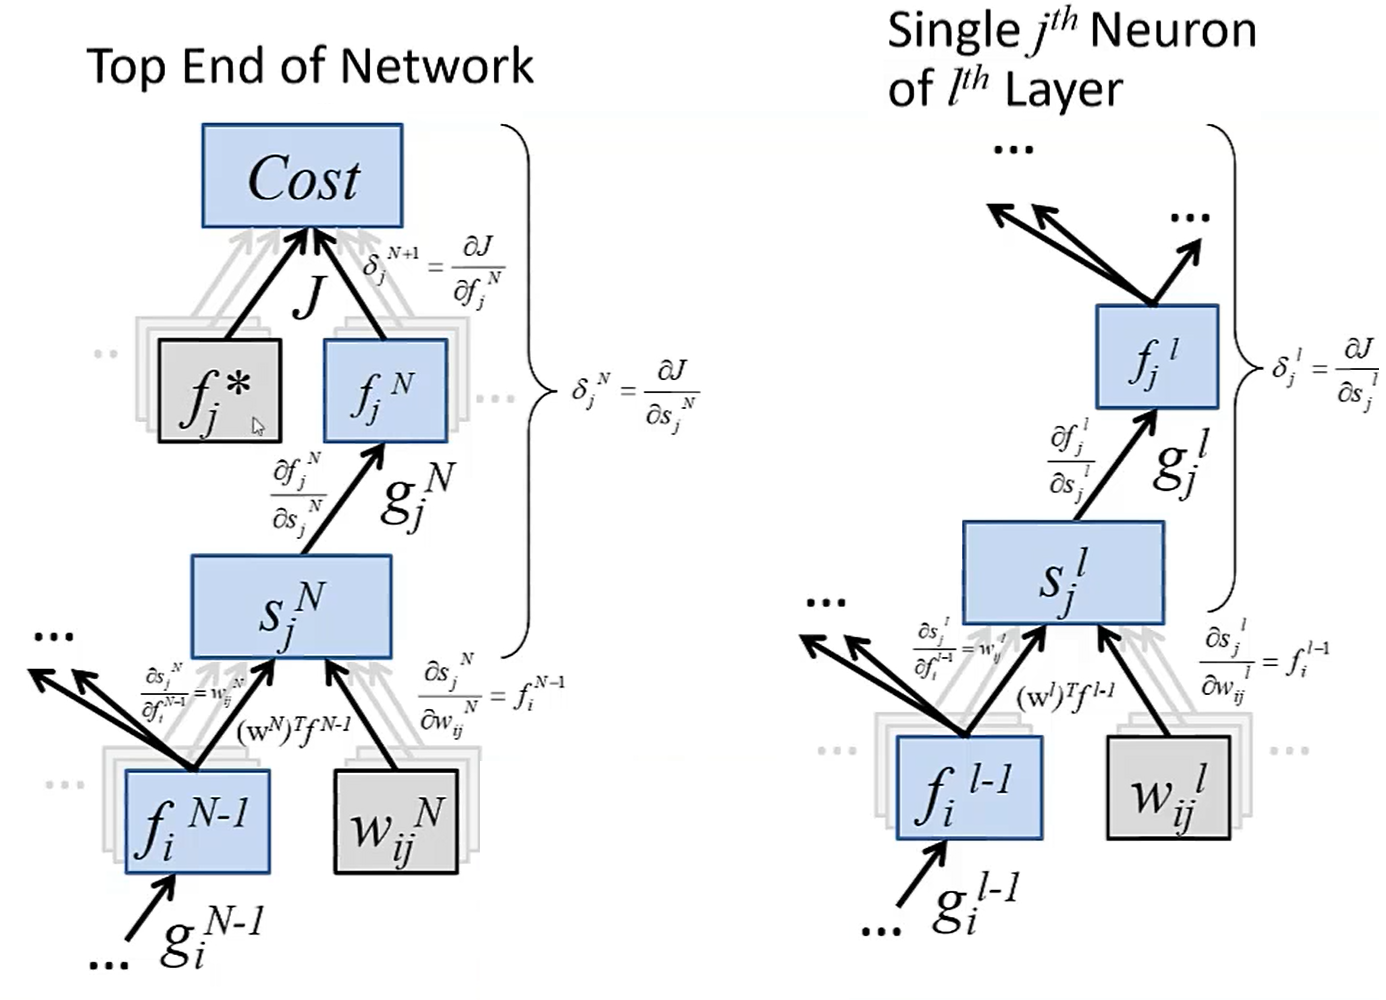
\includegraphics[width=.5\textwidth]{NeuralNetworkComputationalGraph.PNG}
    \caption{Computational Graph of an ANN}
    \label{fig:Computational Graph}
  \end{figure}

  \begin{remark}{\texttt{Figure \ref{fig:Computational Graph}}}
    \begin{itemize}
      \item $J(\cdot,\cdot)$ is the cost function.
      \item $s_j^l:=(w^l)^Tf^{l-1}$ is the signal of the $j^{th}$ node in the $l^{th}$ layer.
      \item $g_j^l(\cdot)$ is the activation function of the $j^{th}$ node in the $l^{th}$ layer.
      \item $f_j^l:=g_j^l(s_j^l)$ is the output of the $j^{th}$ node in the $l^{th}$ layer.
    \end{itemize}
  \end{remark}

\subsection{Backpropagation}

  \begin{definition}{Backpropagation}
    \textit{Backpropagation} is an algorithm for training feedforward neural-networks. \textit{Backpropagation} uses \textit{Reverse Auto-Differentiation} (See \texttt{Section 0.2}) o calculate the derivative of the loss function wrt each weight. The value of the derivative then defines how much to update each weight by.
  \end{definition}

  \begin{proposition}{Backpropagation Algorithm}
    For each training sample $(\mathbf{f}^0,\mathbf{f}^*)$ where $\mathbf{f}^0$ is the input and $\mathbf{f}^*$ is the true output.
    \begin{enumerate}
      \item Read the input \& perform a forward pass through the network to calculate signals $s_j^l$ and outputs $f_j^l$ for all nodes in all layers.
      \[  s_j^l:=(\mathbf{w}_j^l)^T\mathbf{f}^{l-1}\quad f_j^l:=g_j^l(s_j^l) \]

      \item Calculate the cost function value $J(f_j^*,f_j^N)$ between each output layer neuron $f_j^N$ and its target value $f_j^*$.

      \item Calculate the error derivatives $\delta_j^{N+1}$ of the cost function $J$ wrt each output of the last hidden layer $f_j^N$ (ie the values of the output layer).
      \[ \delta_j^{N+1}:=\frac{\partial J}{\partial f_j^N} \]

      \item Compute the error derivative $\delta_j^N$ of the cost function wrt the signals of the last hidden layer $s_j^N$.
      \[ \delta_j^N:=\frac{\partial J}{\partial s_j^N}=g_j^N'(s_j^N)\cdot\delta_j^{N+1} \]

      \item Layer-by-layer: Calculate the \textit{error derivatives} $\delta_i^{l-1}$ of the cost function wrt the signal $s_j^{l-1}$  of each neuron in the next layer, using the error derivatives $\delta_j^l$ of the layer above.
      \[ \delta_i^{l-1}:=\frac{\partial J}{\partial s_i^{l-1}}=g_i^{l-1}'(s_i^{l-1})\sum_{j=1}^{d(l)}w_{ij}^l\delta_j^l \]
      where $d(l)$ is the width of the $l^{th}$ layer.

      \item Calculate the error derivates $\frac{\partial J}{\partial w_{ik}^l}$ wrt to the weights of each neuron $w_{ik}^l$ using the error derivatives of the neuron activities $\delta_j^l$.
      \[ \frac{\partial J}{\partial w_{ij}^l}:=\frac{\partial J}{\partial s_j^l}\frac{\partial s_j^l}{\partial w_{ij}^l}=\delta_j^lf_i^{l-1} \]

      \item Update all weights $w_{ij}^l$ based on the deltas and neuron activities using the \mathit{Gradient Descent} learning rule
      \[ w_{ij}^l\leftarrow w_{ij}^l-\eta f_i^{l-1}\delta_j^l\]
      where $\eta$ is a pre-defined learning rate.
    \end{enumerate}
  \end{proposition}

  \begin{proof}{Derivation of $\delta_i^{l-1}$}
    \everymath={\displaystyle}
    \[\begin{array}{rrl}
      \delta_i^{l-1}&:=&\frac{\partial J}{\partial s_i^{l-1}}\\
      &=&\sum_{j=1}^{d(l)}\underbrace{\frac{\partial J}{\partial s_j^l}}_{\delta_j^l} \underbrace{\frac{\partial s_j^l}{\partial f_j^{l-1}}}_{w_{ij}^l} \underbrace{\frac{\partial f_i^{l-1}}{\partial s_i^{l-1}}}_{g^{l-1}_i'(s_i^{l-1})}\\
      &=&\sum_{j=1}^{d(l)}\delta_j^lw_{ij}^lg_i^{l-1}'(s_i^{l-1})\\
      &=&\underbrace{g_i^{l-1}'(s_i^{l-1})}_\text{independent}\sum_{j=1}^{d(l)}w_{ij}^l\delta_j^l
      \end{array}\]
  \end{proof}

  \begin{definition}{$\nabla J$}
    The derivative for layer $l$ defined below
    \[ \nabla J^l:=\begin{pmatrix}
      f_1^{l-1}\delta_1^l & f_1^{l-1}\delta_2^l & \dots \\
      f_2^{l-1}\delta_1^l & f_2^{l-1}\delta_2^l & \dots \\
      \vdots & \vdots & \ddots
    \end{pmatrix} \] % TODO check rotation/order of elements
  \end{definition}

  \begin{remark}{Limitations with Backpropagation Algorithm}
    Here are some limitations to the \textit{Backpropagation Algorithm}. These are part of the reason why the practice of deep learning did not start earlier.
    \begin{itemize}
      \item The \textit{Vanishing Gradient Problem}. Gradients are unstable/noisy when you backpropagate gradients in a very deep network, meaning that when the true value of the gradient gets very small it is lost in noise.
      \item Descent-based optimisation techniques need to work \underline{accurately and fast} in practice, despite large training data sets. This was not possible before GPU parallelisation and improved optimisers.
      \item Regularisation techniques are critical to achieve good generalisation beyond the training data available (avoid overfitting).
    \end{itemize}
  \end{remark}

  \begin{remark}{Activation Functions need to be Differentiable \& Non-Linear}
    In the \textit{Backpropagation Algorithm} the derivative of each activation function is used, so each activation function must be differentiable.
    \par The step-function does not fulfil this. This is addressed (usually) by using the \textit{ReLU} activation function.
  \end{remark}

\subsection{Gradient Descent}

  \begin{definition}{Gradient Descent}
    \textit{Gradient Descent} is an iterative algorithm for finding a local minimum of a differentiable function. In an ANN this is done by learning a set of weight values $\pmb{w}$ which produce a local minimum for a given cost function $J$. The update rule for gradient descent is
    \[ \pmb{w}_{t+1}=\pmb{w}_t-\underbrace{\eta\cdot\nabla J(X;\pmb{w}_t)}_{\Delta\pmb{w}} \]
    where $\eta$ is a specified learning rate and $\nabla J(X;\pmb{w}_t)$ is the partial derivative of the cost function wrt to the weights (ie the direction of fastest descent). We calculate the $i^\text{th}$ component of $\Delta\pmb{w}$ after observing as $(\pmb{x},f^*(\pmb{x}))$
    \[ [\Delta\pmb{w}]_i=\eta x_i(\underbrace{\pmb{w}^T_t\pmb{x}}_{f(\pmb{x};\pmb{w}_t)}-f^*(\pmb{x})) \]
  \end{definition}

  \begin{definition}{Online Gradient Descent}
    Below is an online algorithm for \textit{Gradient Descent} (ie you can pass it new data without having to restart the process).
    \begin{enumerate}
      \item Initialise all weights $W$ randomly.
      \item \texttt{for each training sample $(x,f^*)$ do}:
      \begin{enumerate}
        \item Forward propagate to calculate network output values.
        \item Back propagate to calculate $\nabla J^l$ for each layer $l$
        \item Update weights for each layer $l$  $W^l\leftarrow W^l-\eta\nabla J^l$.
        \item \texttt{if} (stopping criteria met) \texttt{break loop}.
      \end{enumerate}
      \item \texttt{return} final weights $W^l$ for all layers.
    \end{enumerate}
  \end{definition}

  \begin{definition}{Simulated Annealing}
    \textit{Simulated Annealing} is a process for setting the learning rate $\eta$ by testing $\tau$ learning rates in the interval $[\eta_\tau,\eta_0]$. Annealing transitions from $\eta_0$ to $\eta_\tau$.
    \begin{enumerate}
      \item Initialise all weights $W$ randomly.
      \item \texttt{for} $k=0,\dots,\tau$ \texttt{do}:
      \begin{enumerate}
        \item $\eta_k:=\left(1-\frac{k}\tau)\eta_0+\frac{k}\tau\eta_\tau$
        \item \texttt{for each training sample $(x,f^*)$ do}:
        \begin{enumerate}
          \item Forward propagate to calculate network output values.
          \item Back propagate to calculate $\nabla J^l$ for each layer $l$
          \item Update weights $W^l\leftarrow W^l-\eta_k\nabla J^l$.
          \item \texttt{if} (stopping criteria met) \texttt{break loop}.
        \end{enumerate}
        \item \texttt{return} final weights $W^l$.
      \end{enumerate}
    \end{enumerate}
  \end{definition}

  \begin{remark}{Limitations of \textit{Online Gradient Descent}}
    \begin{itemize}
      \item \textit{Sample Size}. Using single samples at a time to find the minimum point of the cost function will only roughly approximate aspects of the cost function gradient. This leads to a very noisy gradient descent which may not find the global minimum at all. This is exasperated if the learning rate $\eta$ is set too \textit{high} as the minimum may be overshot.
      \par This addressed by \textit{Deterministic Gradient Descent} and \textit{Stochastic Gradient Descent}.
      \item \textit{Constant Learning Rate}. Having the same learning rate $\eta$ for the whole learning process is bad as you cannot skip over shallow gradient, nor focus more iterations in areas of steep gradient. We would rather have weights with a shallow gradient have a greater learning rate, and weights with a steeper gradient have a lesser learning rate.
      \par This is addressed by \textit{Learning via Momentum}.
      \item \textit{Monotonic Learning Rate}. Having the same learning rate $\eta$ for all weights is problematic as weights have different gradients and thus should be learning at different rates as they will hit shallow/steep areas at different times.
      \par This is addressed by \textit{Adaptive Gradient Algorithm} and \textit{Root-Mean-Square Propagation}.
    \end{itemize}
  \end{remark}

\subsubsection{Stochastic \& Deterministic Gradient Descent}

  \begin{definition}{Alternatives to \textit{Online Gradient Descent}}
    As \textit{Online Gradient Descent}'s use of a single sample at a time is bad, multiple samples can be used by using mean $\nabla J$. Here are two approaches
    \begin{itemize}
      \item \textit{Deterministic Gradient Descent} (DGD) where \underline{all} training samples $(X,F^*)$ are used at once. Given a small enough learning rate $\eta$ this will process to the true local minimum, but at high computational cost.
      \item \textit{Stochastic Gradient Descent} (MiniBatch) where a \underline{small subset} of training samples $(X,F^*)$ are used each iteration. This is still good at finding a minimum, and much less computationally costly.
    \end{itemize}
    For the average of $\nabla J$ we use
    \[ \nabla J=\frac1{|X|}\nabla_W\sum_j L(\underbrace{f(\mathbf{x}_j,W)}_\text{\tiny prediction},f^*) \]
  \end{definition}

\subsubsection{Momentum}

  \begin{definition}{Learning via Momentum}
    \textit{Momentum} is a extension to the \textit{Gradient Descent} weight update rule. Rather than a fixed learning rate $\eta$, a velocity term $v_t$ is introduced which defines the step length and direction. The closer the direction of the previous step is aligned to the direction of the current step, the longer the step length is.
    \[ W^l\rightarrow W^l+\underbrace{v^l_{t+1}}_\text{momentum}\quad\text{where}\quad v^l_{t+1}:=\alpha\cdot v^l_t-\eta\nabla J(X;W_t^l) \]
    where $\alpha,\eta$ are hyperparameters for momentum and learning rate, respectively.
  \end{definition}

  \begin{proposition}{Nesterov Accelerated Gradient (NAG)}
    \textit{Nesterov Accelerated Gradient} is an extension of \textit{Learning via Momentum} which, instead of calculating the gradient at the current position, looks-ahead at the gradient of the target. This is since \textit{Momentum} will carry us towards the next location anyway.
    \par Formally we now define weight updates as
    \[ W^l\leftarrow W^l+v^l_{t+1}\quad\text{where}\quad v^l_{t+1}=\alpha v^l_t-\eta\nabla J(X;\underbrace{W^l+\alpha v^l_t}_{ \underset{\text{perview}}{\text{location}}}) \]
    \textit{NAG} is consistently better that \textit{Learning via Momentum} in practice.
  \end{proposition}

  \begin{remark}{Limitations of Momentum Methods}
    Methods which use momentum progress very slowly in shallow plateau regions of the cost function state space as momentum is not able to build up. This can be rectified by tuning the learning rate.
  \end{remark}

  \begin{proposition}{Newton's Method}
    \textit{Newton's Method} removes all hyperparameters ($\eta$ and $\alpha$) and instead uses curvature to rescale the gradient by multiplying the gradient by the inverse Hessian of the current cost function $H(J(X;W_t))$.
    \par \textit{Newton's Method} takes aggressive steps in directions of shallow curvature, and shorter steps in directions of steep curvature, however it is attracted to saddle points (bad!).
    \[ W^l\leftarrow W^l- H(J(X;W^l))^{-1}\nabla J(X;W^l) \]
    \par Computing and inverting the Hessian is computationally and space expensive.
  \end{proposition}

  \begin{remark}{The more parameters there are the more likely saddle points are}
    Saddle points occur when the hessian has both positive \& negative eigenvalues. This is more likely when we have more parameters (as the probability of all eigenvalues being positive is low).
    \par Random Matrix Theory states that the lower the cost function $J$ is (ie the closer it is to the global minimum), the more likely it is to find positive eigenvalues. This means that if we find a minimum it is likely to be a good one (i.e. low cost).
    \par Thus, most critical points with higher cost function values are likely to be saddle points, which we can escape using symmetry-breaking descent methods.
  \end{remark}

\subsubsection{Adaptive Gradient Algorithm (AdaGrad)}

  \begin{definition}{Adaptive Gradient Algorithm (AdaGrad)}
    \textit{Adaptive Gradient Algorithm (AdaGrad)} is an extension to the \textit{Gradient Descent} weight update rule st each weight can have a different learning rate. Scaling the learning rate $\eta$ for each weight wrt the past gradients for that weight.
    \par For each weight $w_i$ the following update rule is used
    \[
      w_i\leftarrow w_i-\frac{\eta g_t}{\sqrt{M_t}+\varepsilon}\quad\text{where}\quad M_t:=\sum_{i=1}^t g_i^2
    \]
    where $\eta$ is a hyper-parameter for the learning rate; $g_t$ is the gradient for this weight in this iteration; $M_t$ is the square-sum of all observed gradients for this weight; and, $\varepsilon>0$ is a small constant to prevent dividing by zero.
  \end{definition}

\subsubsection{Root-Mean-Square Propagation (RMSProp)}

  \begin{definition}{Root-Mean-Square Propagation (RMSProp)}
    \textit{Root-Mean-Square Propagation (RMSProp)} is an extension to the \textit{AdaGrad} weight update rule which introduces a smoothing parameter $\beta$ to combat the aggressive reduction of learning speed.
    \par For each weight $w_i$ the following update rule is used
    \[
      w_i\leftarrow w_i-\frac{\eta g_t}{\sqrt{M_t}+\varepsilon}\quad\text{where}\quad M_t:=(1-\beta) g_t^2+\beta M_{t-1}
    \]
    where $\eta$ is a hyper-parameter for the learning rate; $g_t$ is the gradient for this weight in this iteration; $M_t$ is an  exponentially decaying average\footnote{The influence of each gradient in $M_t$ decays over time. The closer $\beta$ is to $\frac12$ the quicker this occurs.} of the square of all previously observed gradients of this weight; and, $\varepsilon>0$ is a small constant to prevent dividing by zero.
  \end{definition}

\subsubsection{Adaptive Moment Estimation (AdaM)}

  \begin{definition}{Adaptive Moment Estimation (AdaM)}
    \textit{Adaptive Moment Estimation (AdaM)} which aims to smooth the incoming gradient $g_t$ in \textit{RMSProp}. This is done by introducing an exponentially decaying average of all previously observed gradients for this weight $G_t$ (Not just their squares $M_t$)\footnote{$G_t$ is an estimate of the first moment (\textit{ie} mean) of the gradients. $M_t$ is an estimate of the second moments (\textit{ie} un-centred variance) of the gradients.}.
    \par For each weight $w_i$ the following update rule is used
    \everymath={\displaystyle}
    \[\begin{array}{rrl}
      G_t&:=&(1-\alpha)g_t+\alpha G_t\\
      \bar{G}&:=&\frac{G_t}{1-\alpha^{t-1}}\\
      M_t&:=&(1-\beta)g_t^2+\beta M_{t-1}\\
      \bar{M}&:=&\frac{M_t}{1-\beta^{t-1}}\\
      w_i&\leftarrow&w_i-\frac{\eta\bar{G}}{\sqrt{\bar{A}}+\varepsilon}
    \end{array}\]
    where $\alpha,\beta,\eta$ are hyper-parameters for the learning and decay rates; $g_t$ is the gradient for this weight in this iteration; $G_t,M_t$ are an exponentially decaying averages for previously observed gradients of $w_i$, and their squared value; and, $\varepsilon>0$ is a small constant to prevent dividing by zero.
  \end{definition}

  \begin{remark}{$\bar{G}$ and $\bar{M}$}
    $\bar{G}$ forces fast startups. % IDK what that means
    \par Using the square-root of $\bar{M}$ in the update to $w_i$ amplifies shallow gradients (since $\bar{M}$ is small) and dampens steep gradients (since $\bar{M}$ is large).
  \end{remark}

  \begin{remark}{Using AdaM}
    Applying AdaM to a ReLU-based network is sufficient to perform deep learning but there are other features which need to be decided.
    \begin{enumerate}
      \item What to set hyperparameters $\alpha,\beta,\varepsilon$ and the size of each training batch.
      \item How to initialise the network.
      \item How to avoid overfitting.
      \item Which loss function to use.
    \end{enumerate}
    Tuning and trial-and-error of these features is often required to achieve good results from deep learning.
  \end{remark}

\subsection{Cost Function}

  \begin{definition}{Cost Function, $J(\cdot,\cdot)$}
    A \textit{Cost Function} is a real-valued measure of how inaccurate a classifier is for a given input configure (\textit{ie} test data $[X,f^*(X)]$ and weights $W$). Greater values imply the classifier is less accurate.
    \par Neural networks us training to learn a set of weights which minimise the \textit{Cost Function}, given the training data.
  \end{definition}

\subsubsection{Numerical}

  \begin{proposition}{Distance Measures for Numerical Quantities $L(\cdot,\cdot)$}
    Let $x,x^*\in\reals$ with $x$ representing an estimate and $x^*$ the true value.
    \par Here are some popular measures of distance between real-valued quantities.
    \begin{itemize}
      \item[\textit{Identity Distance}] $L(x,x^*):=|x-x^*|$
      \item[\textit{Absolute Distance}] $L(x,x^*):=(x-x^*)^2$
      \item[\textit{Quadratic Distance}] $L(x,x^*):=\identity\{x\equiv x^*\}=\begin{cases}1&\text{if }x\equiv x^*\\0&\text{otherwise} \end{cases}$
    \end{itemize}
  \end{proposition}

  \begin{proposition}{Cost Functions for Numerical Quantities $J$}
    Let $[X,f^*(X)]$ be a set of training data, $f_W(\cdot)$ be the values our model predicts when using weight set $W$ and $L(\cdot,\cdot)$ be some \textit{Loss Function}.
    \par Here are some \textit{Cost Functions} for classifiers which classify real-valued quantities.
    \begin{itemize}
      \item[\textit{Expected Loss}] $\displaystyle J(X;W)=\expect[L(f_W(X),f^*(X))]$
      \item[\textit{Empirical Risk}] $\displaystyle J(X;W)=\frac1{|X|}\sum_{\x\in X}L(f_W(\x),f^*(\x))$
    \end{itemize}
  \end{proposition}

\subsubsection{Classification}

  \begin{remark}{Non-Numerical Cost Measures}
    In non-numerical classification there is no obvious way to define the distance between classification. Thus we cannot define a cost function.
    \par How we combat this depends on how the output layer is defined. When using the setup of the output layer defined in \texttt{Proposition 4.2}, which uses \textit{Softmax}, the \textit{Cross-Entropy Cost Function Function}
  \end{remark}

  \begin{definition}{Cross-Entropy Cost Function $J$}
    Let $f_j^*$ be the ground truth for output node $j$ and $f_j^N$ be our predicted value for the ground truth for output node $j$.
    \par The \textit{Cross-Entropy Cost Function} $J$ and its derivative $\delta_i^N$ wrt signal $i$ is defined as
    \[\begin{array}{rrl}
    J&:=&-\displaystyle\sum_{j\in\text{Group}}f_j^*\ln(f_j^N)\\
    \delta_i^N&=&f_i^N-f_i^*
    \end{array}\]
    The cost function derivative $\delta_i^N$ is just the difference between the predicted value and the true value.
  \end{definition}

  \begin{proof}{Derivation of Derivative $\delta_i^N$ of Cross-Entropy Cost Function}
    The steepness of the cost function derivative $\frac{\partial J}{\partial f_j^N}$ exactly cancels the shallowness of the softmax derivative $\frac{\partial f_j^N}{\partial s_i^N}$, leading to an \textit{MSE-Style Delta} $\delta_i^N$ which is propagated backwards from layer $N$.
    \everymath={\displaystyle}
    \[\begin{array}{rrl}
      \delta_i^N&:=&\frac{\partial J}{\partial s_i^N}\\
      &=&-\sum_{j\in\text{Group}}f_j^*\underbrace{\frac{\partial \ln(f_j^N)}{\partial s_i^N}}_\text{apply chain rule}\\
      &=&-\sum_{j\in\text{Group}}f_j^*\frac1{f_j^N}\frac{\partial f_j^N}{\partial s_i^N}\quad\text{where }f_j^N:=\frac{e^{s_j^N}}{\sum_{i\in\text{Group}}e^{s_i^N}}\\
      &=&-\sum_{j=i}f_j^*\frac1{f_j^N}\underbrace{f_j^N(1-f_j^N)}_{\frac{\partial f_j^N}{\partial s_i^N}\text{ for }i=j}-\sum_{j\neq i}f_j^*\frac1{f_j^N}\underbrace{(-f_j^Nf_i^N)}_{\frac{\partial f_j^N}{\partial s_i^N}\text{ for }i\neq j}\\
      &=&-f_i^*(1-f_i^N)+\sum_{j\neq i}f_j^*\frac{f_j^Nf_i^N}{f_j^N}\\
      &=&-f_i^*+\underbrace{f_i^*f_i^N+\sum_{j\neq i}f_j^*f_i^N}_{=f_i^N\sum_{j\in\text{Group}}f_j^*}\\
      &=&f_i^N\underbrace{\left(\sum_{j\in\text{Group}}f_j^*\right)}_{=1}-f_i^*\\
      &=&f_i^N-f_i^*
    \end{array}\]
  \end{proof}

\newpage
\setcounter{section}{-1}
\section{Reference}

  \begin{definition}{Convolution $*$}
    \textit{Convolution} is an operation which takes two functions $f$ \& $g$ and produces a third function $(f*g)$ which shows how one function affects the other.
    \par Consider the 2D discrete space where $f,g$ are real valued 2D matrices (often representing images). \textit{Convolution} in this case is defined as
    \[ (f*g)(x,y)=\sum_{i\in I}\sum_{j\in J}f(x-i,y-j)\cdot g(i,j) \]
    where $I$ is the horizontal index of $g$ and $J$ is the vertical index of $g$.
    \par Typically a \textit{Convolution} is then shift right until the RHS of the kernel surpasses the RHS of the input, it will then shift down a row. This will continue until the bottom row has been completed
    \begin{center}
      \includegraphics[width=.35\textwidth]{2dConvolution.PNG}
    \end{center}
    Note that \textit{Convolution} reduces the size of the input. To avoid this \textit{Zero-padding} is used, where a ring on zeros is placed around the input.
  \end{definition}

  \begin{definition}{Hessian Matrix $H(\cdot)$}
    \[ H(J)=\begin{pmatrix}\frac{\partial J^2}{\partial w_1^2}&\frac{\partial J^2}{\partial w_1\partial w_2}&\dots&\frac{\partial J^2}{\partial w_1\partial w_n}\\\frac{\partial J^2}{\partial w_2\partial w_1}&\frac{\partial J^2}{\partial w_2^2}&\dots&\frac{\partial J^2}{\partial w_2\partial w_n}\\\vdots&\vdots&\ddots&\vdots\\\frac{\partial J^2}{\partial w_n\partial w_1}&\frac{\partial J^2}{\partial w_n\partial w_2}&\dots&\frac{\partial J^2}{\partial w_n^2}\end{pmatrix}\]
  \end{definition}

\subsection{Feed-Forward Network}

  \begin{definition}{Feed-Forward Network}
    A \textit{Feed-Forward Network} is an artificial neural network where the connections between nodes are uni-directional. Data is provided to the input layer and then an output is returned from the output layer, no layers are visited twice.
  \end{definition}

\subsection{Auto-Differentiation}

  \begin{figure}[H]
    \centering
    \subfloat[Equations]{
      \[\begin{array}{rclc}
        a&=&b\times c\\
        b&=&d+e\\
        c&=&e+2\\
        d&=&3+f\\
        e&=&f\times g
      \end{array}\]
    }
    \subfloat[Graph]{
      \begin{tikzpicture}
        % nodes
        \node[circle] at (0,0)   (3) {$3$};
        \node[circle] at (0,-2)  (f) {$f$};
        \node[circle] at (0,-4)  (g) {$g$};

        \node[circle] at (2,-1)  (d) {$d:=3+f$};
        \node[circle] at (2,-3)  (e) {$e:=f\times g$};
        \node[circle] at (2,-5)  (2) {$2$};

        \node[circle] at (4,-2)  (b) {$b:=d+e$};
        \node[circle] at (4,-4)  (c) {$c:=e+2$};

        \node[circle] at (6,-3)  (a) {$a:=b\times c$};

        % edges
        \path[->]
        (3) edge (d)
        (f) edge (d)
        (f) edge (e)
        (g) edge (e)

        (d) edge (b)
        (e) edge (b)
        (e) edge (c)
        (2) edge (c)

        (b) edge (a)
        (c) edge (a)
        ;
      \end{tikzpicture}
    }
    \caption{Example of a Feedforward Computational Graph}
    \label{fig:Feedforward_Computational_Graph}
  \end{figure}

\begin{figure}[H]
  \begin{center}
    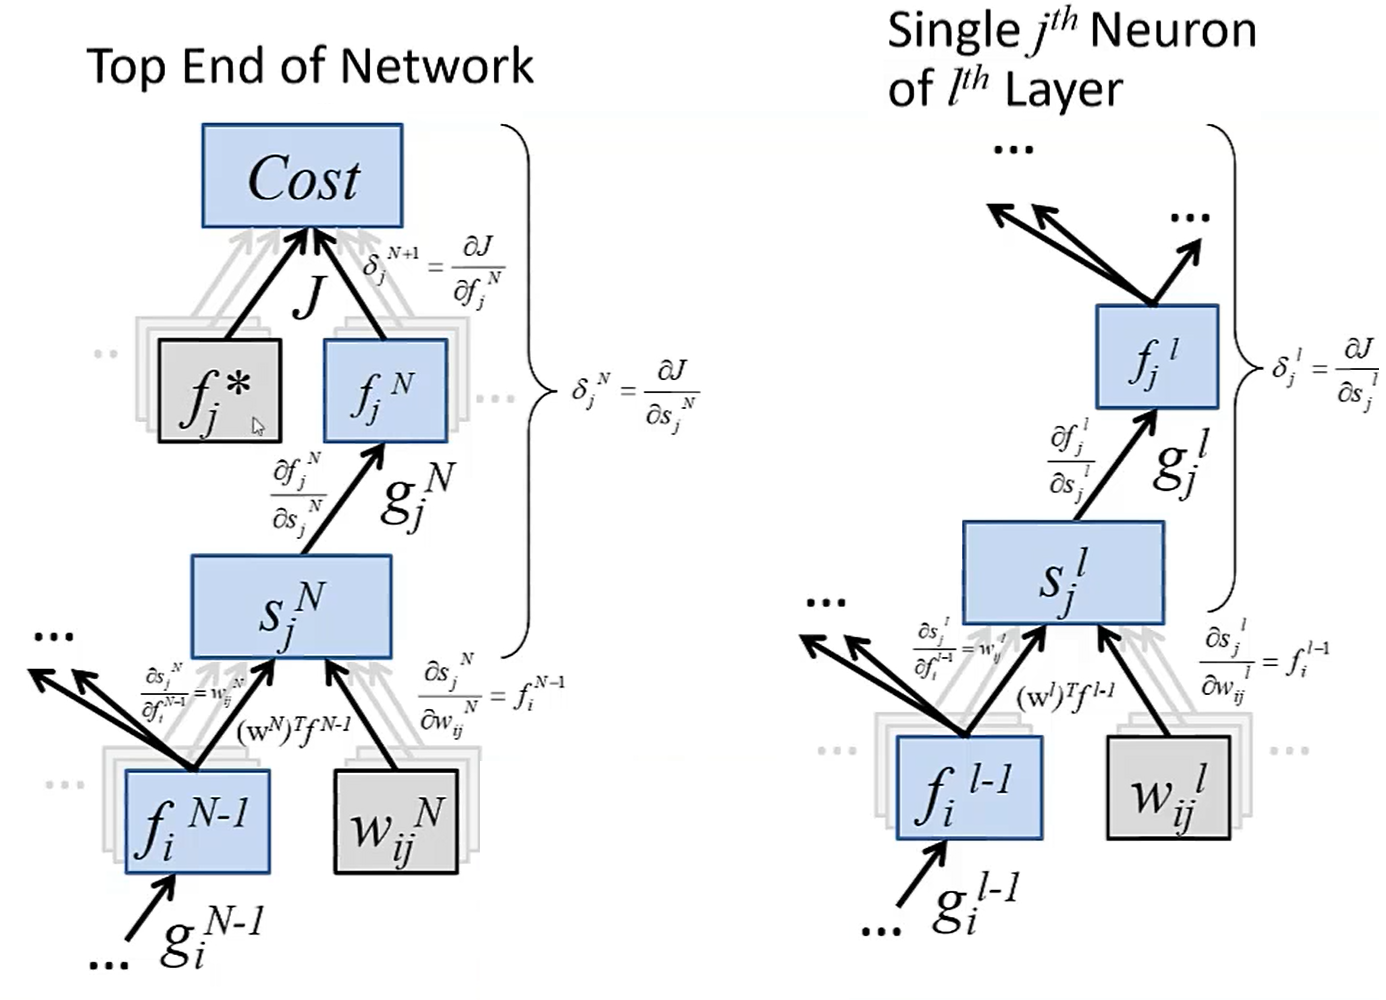
\includegraphics[width=.7\textwidth]{NeuralNetworkComputationalGraph.PNG}
  \end{center}
  \caption{A Neural Network as a Feedforward Computational Graph.\\ \footnotesize{$J$ is the cost function, $s_j^l,\ g_j^l(\cdot),\ f_j^l$ are the signal, activation function and output of the $j^{th}$ node in the $l^{th}$ layer respectively.} }
  \label{fig:NN_Feedforward_Computational_Graph}
\end{figure}

  \begin{definition}{Feedforward Computational Graph}
    A \textit{Feedforward Compurational Graph} is a uni-directional graph which represents a series of equations. In a \textit{Feedfoward Computational Graph} nodes represent variables or constants and edges represent mathematical operations (and thus dependence between nodes).
    \par If values are set for all leaves of the graph, then values can be calculated for all nodes in the graph. Moreover, if values are defined for all nodes at a given depth then values can be calculate for all variables higher up the tree.
    \par \texttt{Figure \ref{fig:Feedforward_Computational_Graph}} provides an example of a \textit{Feedforward Computational Graph}.
  \end{definition}

  \begin{definition}{Auto-Differentiation}
    \textit{Auto-Differentiation} is a technique for calculating partial derivatives of a \textit{Feedforward Computational Graph} and is used by \textit{Gradient Descent}.
    \par Consider two nodes in a computational graph $x,y$. Use the following process to calculate the partial derivative $\frac{\partial x}{\partial y}$.
    \begin{enumerate}
      \item Establish all the paths from $y$ to $x$ in the graph.
      \item Calculate the partial derivatives of each step of these graphs. (i.e. if there is a path $y\to a\to x$ calculate $\frac{\partial a}{\partial y},\frac{\partial x}{\partial a}$).
      \item Apply the chain rule along each path (i.e. For $y\to a\to x$ calculate $\frac{\partial a}{\partial y}\cdot\frac{\partial x}{\partial a}$).
      \item Sum these calculations together to get the final result $\frac{\partial x}{\partial y}$.
      \item Substitute variables to make computation easier.
    \end{enumerate}
  \end{definition}

  \begin{example}{Auto-Differentiation using a Feedforward Computational Graph}
    Consider calcualte $\frac{\partial f}{\partial a}$ for the graph in  \texttt{Figure \ref{fig:Feedforward_Computational_Graph}}.
    \begin{enumerate}
      \item There are three paths from $f$ to $a$ in the graph: (1) $f\to d\to b\to a$; (2) $f\to e\to b\to a$; and, (3) $f\to e\to c\to a$.
      \item We need to calculate the following sets of partial derivatives: $\frac{\partial d}{\partial f},\frac{\partial b}{\partial d},\frac{\partial a}{\partial b}$ for (1); $\frac{\partial e}{\partial f},\frac{\partial b}{\partial e},\frac{\partial a}{\partial b}$ for (2); and, $\frac{\partial e}{\partial f},\frac{\partial c}{\partial e},\frac{\partial a}{\partial c}$ for (3).
      \[\begin{array}{rclcrclcrcl}
        &(1)&&&&(2)&&&&(3)\\
        \frac{\partial d}{\partial f}&=&1&\quad&\frac{\partial e}{\partial f}&=&g&\quad&\frac{\partial e}{\partial f}&=&g\\
        \frac{\partial b}{\partial d}&=&1&\quad&\frac{\partial b}{\partial e}&=&1&\quad&\frac{\partial c}{\partial e}&=&1\\
        \frac{\partial a}{\partial b}&=&c&\quad&\frac{\partial a}{\partial b}&=&c&\quad&\frac{\partial a}{\partial c}&=&b
      \end{array}\]
      \item Applying the chain rule to each path gives
      \[\begin{array}{rrcl}
        (1)&\frac{\partial d}{\partial f}\frac{\partial b}{\partial d}\frac{\partial a}{\partial b}&=&1\cdot1\cdot c=c\\
        (2)&\frac{\partial e}{\partial f}\frac{\partial e}{\partial f}\frac{\partial b}{\partial e}&=&g\cdot1\cdot1\cdot c=gc\\
        (3)&\frac{\partial e}{\partial f}\frac{\partial c}{\partial e}\frac{\partial a}{\partial c}&=&g\cdot1\cdot b=gb\\
      \end{array}\]
      \item Summing the terms together we get
      \[ \frac{\partial a}{\partial f}=c+gc+gb \]
      \item By substitution we get a final expression
      \[ \frac{\partial a}{\partial f}=2+5g+2fg+2fg^2 \]
    \end{enumerate}
    So when $f=4,g=2$ we have that $a=150$ and $\frac{\partial a}{\partial f}=60$.
  \end{example}

  \begin{proposition}{Using Hierarchical Dependency}
    By the chain rule we have that $\frac{\partial x}{\partial z}=\frac{\partial x}{\partial y}\frac{\partial y}{\partial z}$. So, if $\frac{\partial x}{\partial y}$ is already known then we just need to multiply that value by $\frac{\partial y}{\partial z}$ to get $\frac{\partial x}{\partial z}$.
    \par This can be utilised to ease the computational load of a calculation. In particular, calculating the derivatives one layer at a time is a good strategy.
  \end{proposition}

  \begin{remark}{Usefulness of Auto-Differentiation}
    \textit{Auto-Differentiation} allows us to mathematical quantify the affect one variable has on another, which is good. However, the number of paths in a network grows exponentially with the number of nodes, thus this can be computational hard. (\textit{Hierarchical Dependence} can be used to mitigate this)
  \end{remark}

\end{document}
